\section{Results and discussion}

\subsection{Flow in a channel}

\begin{figure}[H]
    \centering
    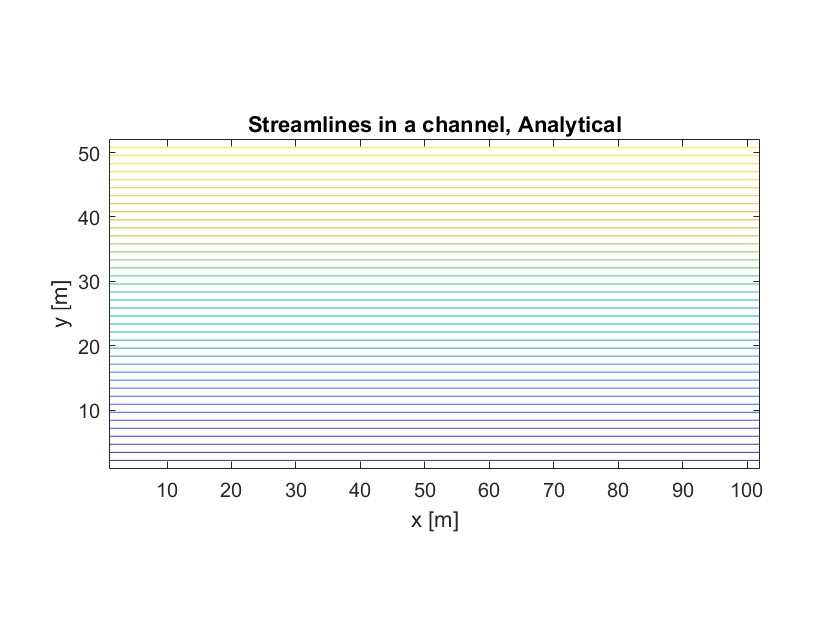
\includegraphics[width=0.7\linewidth]{imatges/strmchannelanal.jpg}
    \caption{Streamlines for the analytical solution of flow in a channel.}
    \label{fig:nocilinderanalytical}
\end{figure}

\begin{figure}[H]
    \centering
    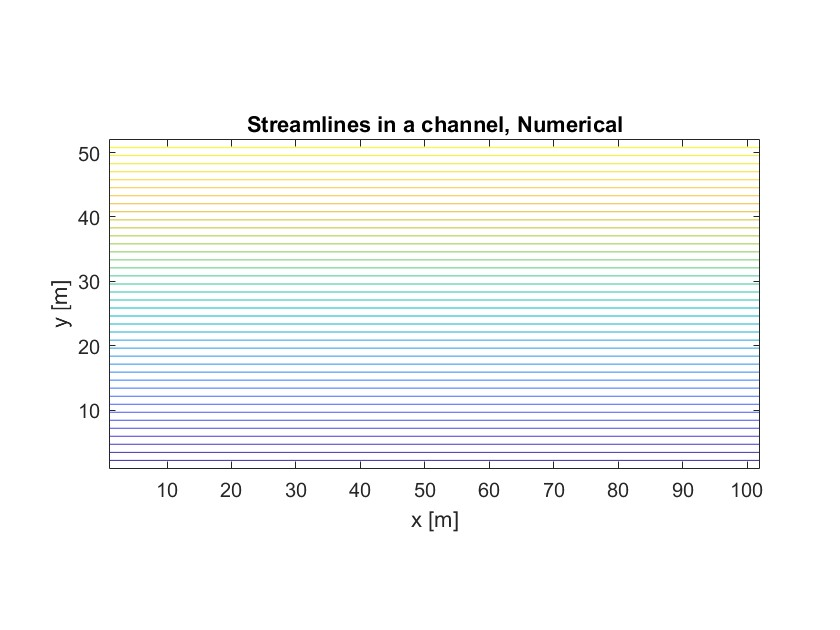
\includegraphics[width=0.7\linewidth]{imatges/strmchannelnum.jpg}
    \caption{Streamlines for the numerical solution of flow in a channel.}
    \label{fig:nocilindernumerical}
\end{figure}

Converged in 11123 iterations with residual = 9.988526e-10

The provided figures compare the analytical and numerical solutions of flow streamlines in a channel. The analytical solution in Figure \ref{fig:nocilinderanalytical} exhibits a uniform and parallel flow pattern, which is expected for an idealized potential flow in a channel, with no visible disturbances, suggesting a perfect theoretical model with constant velocity distribution. In contrast, the numerical solution in Figure \ref{fig:nocilindernumerical} also demonstrates fairly parallel streamlines, indicating a good numerical approximation. Overall, the numerical solution closely matches the analytical one, confirming that the numerical method is correctly implemented.
